\documentclass[12pt,a4paper]{article}
% 12pt:     Tamaño de fuente
% a4papper: Tamaño de papel
% article:  Formato artículo, está dividido por secciones y subsecciones. Otros formatos: report, letter, book, etc.

\usepackage[spanish, es-tabla]{babel}
% Configura en español los nombres de figuras, tablas, etc.
\usepackage[utf8]{inputenc}                 % Permite el uso directo de tildes y otros.
\usepackage{amsmath,amssymb}
% Añade símbolos matemáticos para las ecuaciones.
\usepackage{parskip}
% Elimina la sangría
\usepackage{geometry}
% Permite modificar los márgenes de la página a gusto.
\usepackage{multicol}
% Ordena el cuerpo del documento en 2 o más columnas.
\usepackage{graphicx}
% Para poner imágenes.
\usepackage{enumitem}
% Para modificar los tags de los enumerate.
\usepackage{array}
% Para ordenar texto y ecuaciones.
\usepackage{url}
% Permite usar url que redirigen a la página web.
\usepackage{hyperref}
% Permite que se puedan clickear las urls, citas y referencias.

\spanishdecimal{.} % punto decimal
\geometry{margin=2cm} % margenes de la hoja
\renewcommand{\baselinestretch}{1.3} % tamaño de las filas de las tablas

\begin{document}

\begin{center}
{\Large\textbf{INFORME N°1}}

{\LARGE\textbf{Fundamentos de Medición, Tratamiento de Errores}}
{\LARGE\textbf{y Análisis de Datos}}

\rule{\textwidth}{0.5pt}

\begin{tabular}{ll}
    \textbf{Estudiantes:} & Benjamín Moraga \\
                          & Ian Barra \\
                          & Juan Ortega \\
                          & Nicolás Saldivia \\
                          & Mauricio Ortega \\ [0.2cm] 
    \textbf{Profesora:}   & Constanza Rivas \\
    \textbf{Ayudante:}    & Annelies Fullgraff \\[0.2cm]
    \textbf{Fecha de entrega:} & 28 de Agosto de 2026
\end{tabular}

\vspace{0.4cm}
\rule{\textwidth}{0.5pt}

\end{center}

\section{Parte 1 - Medición directa de magnitudes físicas} \label{Parte-1}

\subsection{Procedimiento experimental} \label{Procedimiento-Parte-1}

\begin{enumerate}[label=\alph*)]
\item Los objetos y magnitudes que hemos medido son: El diametro de un plumón, el largo de un plumón, el grosor de una de las mesas del laboratorio, el tiempo de caida de una hoja de papel desde la mesa del laboratorio hasta el piso y el grosor de un pelo de uno de los integrantes.
\item Para medir el diametro del plumón utilizamos el pie de metro, pues la escala es la adecuada y además se facilitó bastante técnicamente realizar la medición. Para medir el largo del plumón volvimos a utilizar el pie de metro, pues realizar la medición fue bastante comodo con ese instrumento, ya que agarra el plumón de ambos extremos, mejorando la precisión de la medida.
   Para medir el grosor de la mesa del laboratorio usamos una regla ya que cuenta con la precisión necesario y fue comodo realizar las mediciones. Para medir el tiempo de caida de la hoja usamos un cronómetro, simplemente es un buen instrumento para medir el tiempo de manera práctica. Parar medir el grosor del cabello, utilizamos el micrómetro, pues la escala es la adecuada 
   ya que el grosor de un cabello es tan pequeño que usar una regla o un pie de metro seria poco exacto. 
\item Con todos los objetos seleccionados hicimos lo mismo, dos mediciones cada integrante del grupo y las fuimos anotando. Para el diametro del plumón utilizamos el pie de metro y ajustamos al grosor del plumón. Para el largo del plumón lo mismo, pusimos el pie de metro a lo largo del plumon, ajustandolo en cada extremo de el.
   Para el grosor de la mesa pusimos la regla en distintas partes del grosor de la mesa, dandonos unas medidas bastante precisas. Para medir el tiempo de caida de la hoja, uno de los integrantes del grupo deja caer la hoja desde la altura de la mesa, justo en ese momento se acciona el cronómetro y cuando cae, se vuelve a accionar, dando el tiempo de caída de la hoja,
   aunque esa medición es bastante poco precisa, pues depende de diversos factores los cuales se hizo complicado controlar. Para medir el grosor del cabello simplemente lo pusimos en el micrómetro y lo ajustamos, dandonos medidas un poco variadas ya que tal vez algunos ajustaban un poco más y otros un poco menos.
\item Cada uno realizó dos mediciones de cada magnitud, y cada uno anotó todas las mediciones de uno de los objetos
\item Siempre procuramos tener una organización clara a la hora de medir las magnitudes y nos preocupamos de realizar de manera correcta las medidas
\item No descartamos ni repetimos ninguna de las mediciones, sin embargo a la hora de medir el tiempo de caída de la hoja lo pensamos pero vimos que era normal que hubiera bastante variación en las medidas.
\end{enumerate}

 En las subsecciones siguientes, presenten los resultados y cálculos correspondientes a cada conjunto de mediciones y hagan referencia a esta sección cuando sea necesario.
\subsection{Cálculos realizados}

Para calcular el promedio $\bar{x}$ se realizó el siguiente procedimiento:

\begin{align*}
\bar{x} &= \frac{1}{N} \sum_{i=1}^{N} x_i 
\end{align*}

\begin{itemize}
\item $\bar{x}_{diametroPlumon} =  $
\item $\bar{x}_{largoPlumon} = 13,406~cm$
\item $\bar{x}_{grosorMesa} = 0,020~m$
\item $\bar{x}_{tiempoHoja} = 1,179~s$
\item $\bar{x}_{grosorCabello} = 0,063~mm $

\end{itemize}

\bigskip

Luego, para calcular la desviación estándar $s$ se realizó el siguiente procedimiento:

\begin{align*}
s &= \sqrt{\frac{1}{N-1} \sum_{i=1}^{N} (x_i - \bar{x})^2}
\end{align*}

\begin{itemize}
\item $s_{diametroPlumon}= $
\item $s_{largoPlumon}= 0,057~cm$
\item $s_{grosorMesa}= 0,0011~m$
\item $s_{tiempoHoja}= 0,489~s$
\item $s_{grosorCabello}= 0,026~mm$
\end{itemize}



Finalmente, para calcular el error relativo porcentual $\varepsilon_{x\%}$ se realizó el siguiente procedimiento:

\begin{align*}
\varepsilon_{x\%} &= \left(\frac{\Delta x}{\bar{x}}\right) \times 100
\end{align*}

\begin{itemize}
\item $\varepsilon_{x\%diametroPlumon}= $
\item $\varepsilon_{x\%largoPlumon}= 0,42\%$
\item $\varepsilon_{x\%grosorMesa}= 4,81\%$
\item $\varepsilon_{x\%tiempoHoja}= 41,5\%$
\item $\varepsilon_{x\%grosorCabello}= 41,2\%$
\end{itemize}


\subsection{Nombre del primer instrumento}

Escriban una breve descripción del objeto, indicando sus características físicas y geométricas. El conjunto de todas las mediciones realizadas sobre \textit{la magnitud} del objeto puede encontrarse en la Tabla \ref{mediciones-inst-1}.

\begin{multicols}{3}
\begin{itemize}
    \item Objeto:
    \item Magnitud:
    \item Resolución instrumento:
\end{itemize}
\end{multicols}

\begin{table}[h!]
\centering
\begin{tabular}{|c|c|}
\hline
\textbf{Medición N°} & \textit{Magnitud} \textbf{(}\textit{Unidad}\textbf{)} \\ \hline
1 & \\ \hline
2 & \\ \hline
3 & \\ \hline
\vdots & \\ \hline
\textbf{Promedio $\bar{x}$} & \\ \hline
\textbf{Desviación Estándar $s$} & \\ \hline
\textbf{Error absoluto $\Delta x$} & \\ \hline
\textbf{Error Relativo Porcentual $\varepsilon_{x\%}$} & \\ \hline
\end{tabular}
\caption{Conjunto de mediciones y los respectivos cálculos realizados con \textit{el instrumento} sobre \textit{la magnitud} de \textit{el objeto}.}
\label{mediciones-inst-1}
\end{table}


Así, con los cálculos realizados sobre los datos disponibles en la Tabla \ref{mediciones-inst-1}, se llegó a que \textit{la magnitud} de \textit{el objeto} es:

\begin{equation*}
x = \bar{x} \pm \Delta x
\end{equation*}

\subsection{pie de metro}

El segundo objeto elegido fue un plumon de pizzarra, el cual tiene una figura parecida a la de un cilindro y es blanco con tapa azul. El conjunto de todas las mediciones realizadas sobre el \textit{largo} del objeto puede encontrarse en la Tabla \ref{mediciones-inst-2}.

\begin{multicols}{3}
\begin{itemize}
    \item Objeto: \\ Plumón
    \item Magnitud: \\ Largo
    \item Resolución instrumento: \\ pie de metro 
\end{itemize}
\end{multicols}

\begin{table}[h!]
\centering
\begin{tabular}{|c|c|}
\hline
\textbf{Medición N°} & \textit{distancia} \textbf{(}\textit{cm}\textbf{)} \\ \hline
1 & 13,325 $\pm$ 0,00005 \\ \hline
2 & 13,460 $\pm$ 0,00005 \\ \hline
3 & 13,330 $\pm$ 0,00005 \\ \hline
4 & 13,350 $\pm$ 0,00005 \\ \hline
5 & 13,390 $\pm$ 0,00005 \\ \hline
6 & 13,440 $\pm$ 0,00005 \\ \hline
7 & 13,470 $\pm$ 0,00005 \\ \hline
8 & 13,480 $\pm$ 0,00005 \\ \hline
9 & 13,400 $\pm$ 0,00005 \\ \hline
10 & 13,420 $\pm$ 0,00005 \\ \hline
\textbf{Promedio $\bar{x}$} & 13,406 \\ \hline
\textbf{Desviación Estándar $s$} & 0,057 \\ \hline
\textbf{Error absoluto $\Delta x$} & 0,057 \\ \hline
\textbf{Error Relativo Porcentual $\varepsilon_{x\%}$} & 0,42\% \\ \hline
\end{tabular}
\caption{Conjunto de mediciones y los respectivos cálculos realizados con el \textit{pie de metro} sobre el \textit{largo} del \textit{plumón}.}
\label{mediciones-inst-2}
\end{table}

Siguiendo el mismo procedimiento que para el objeto anterior, esta vez con los datos disponibles en la Tabla \ref{mediciones-inst-2}, se llegó a que el \textit{largo} del \textit{plumón} es:

\begin{equation*}
x = 13,406 \pm 0,00005 \textrm{cm}
\end{equation*}

\subsection{Regla}

El tercer objeto elegido fue el tablero de una de las mesas del laboratorio, esta es de amplia superficie, de madera y un grosor de algunos centimetros. El conjunto de todas las mediciones realizadas sobre \textit{el grosor} del objeto puede encontrarse en la Tabla \ref{mediciones-inst-3}.

\begin{multicols}{3}
\begin{itemize}
    \item Objeto: \\ Mesa
    \item Magnitud: \\ Grosor
    \item Resolución instrumento: \\ 0,001 m
\end{itemize}
\end{multicols}

\begin{table}[h!]
\centering
\begin{tabular}{|c|c|}
\hline
\textbf{Medición N°} & \textit{distancia} \textbf{(}\textit{m}\textbf{)} \\ \hline
1 & 0,0210 $\pm$ 0,0005 \\ \hline
2 & 0,0210 $\pm$ 0,0005 \\ \hline
3 & 0,0210 $\pm$ 0,0005 \\ \hline
4 & 0,0210 $\pm$ 0,0005 \\ \hline
5 & 0,0210 $\pm$ 0,0005 \\ \hline
6 & 0,0210 $\pm$ 0,0005 \\ \hline
7 & 0,0210 $\pm$ 0,0005 \\ \hline
8 & 0,0210 $\pm$ 0,0005 \\ \hline
9 & 0,0190 $\pm$ 0,0005 \\ \hline
10 & 0,0190 $\pm$ 0,0005 \\ \hline
\textbf{Promedio $\bar{x}$} & 0,020 \\ \hline
\textbf{Desviación Estándar $s$} & 0,0011 \\ \hline
\textbf{Error absoluto $\Delta x$} & 0,001 \\ \hline
\textbf{Error Relativo Porcentual $\varepsilon_{x\%}$} &  4,81\% \\ \hline
\end{tabular}
\caption{Conjunto de mediciones y los respectivos cálculos realizados con la \textit{regla} sobre el \textit{grosor} de la \textit{mesa}.}
\label{mediciones-inst-3}
\end{table}

Siguiendo el mismo procedimiento que para el objeto anterior, esta vez con los datos disponibles en la Tabla \ref{mediciones-inst-3}, se llegó a que \textit{la magnitud} de \textit{el objeto} es:

\begin{equation*}
x = 0,020 \pm 0,001\textrm{m}
\end{equation*}

\subsection{cronómetro}

El cuarto objeto es una hoja de papel, delgada, amplia y facil de deformar. El conjunto de todas las mediciones realizadas sobre \textit{la magnitud} del objeto puede encontrarse en la Tabla \ref{mediciones-inst-4}.

\begin{multicols}{3}
\begin{itemize}

    \item Objeto: \\ Hoja de papel
    \item Magnitud: \\ Tiempo de caida
    \item Resolución instrumento: \\ 0,015 seg
\end{itemize}
\end{multicols}

\begin{table}[h!]
\centering
\begin{tabular}{|c|c|}
\hline
\textbf{Medición N°} & \textit{tiempo} \textbf{(}\textit{s}\textbf{)} \\ \hline
1 & 0,970 $\pm$ 0,0055 \\ \hline
2 & 0,910 $\pm$ 0,0055 \\ \hline
3 & 2,470 $\pm$ 0,0055 \\ \hline
4 & 0,790 $\pm$ 0,0055 \\ \hline
5 & 1,040 $\pm$ 0,0055 \\ \hline
6 & 0,930 $\pm$ 0,0055 \\ \hline
7 & 0,870 $\pm$ 0,0055 \\ \hline
8 & 1,180 $\pm$ 0,0055 \\ \hline
9 & 1,350 $\pm$ 0,0055 \\ \hline
10 & 1,280 $\pm$ 0,0055 \\ \hline
\textbf{Promedio $\bar{x}$} & 1,179 \\ \hline
\textbf{Desviación Estándar $s$} & 0,489 \\ \hline
\textbf{Error absoluto $\Delta x$} & 0,489 \\ \hline
\textbf{Error Relativo Porcentual $\varepsilon_{x\%}$} & 41,5\% \\ \hline
\end{tabular}
\caption{Conjunto de mediciones y los respectivos cálculos realizados con el \textit{cronómetro} sobre el \textit{tiempo de caida} de la \textit{hoja de papel}.}
\label{mediciones-inst-4}
\end{table}

Siguiendo el mismo procedimiento que para el objeto anterior, esta vez con los datos disponibles en la Tabla \ref{mediciones-inst-4}, se llegó a que \textit{la magnitud} de \textit{el objeto} es:

\begin{equation*}
x = 1,179 \pm 0,026 \textrm{s}
\end{equation*}

\subsection{Micrómetro}

El quinto objeto elegido fue un cabello, Este es delgado, largo y bastante ligero. El conjunto de todas las mediciones realizadas sobre \textit{el grosor} del objeto puede encontrarse en la Tabla \ref{mediciones-inst-5}.

\begin{multicols}{3}
\begin{itemize}
    \item Objeto: \\ Cabello
    \item Magnitud: \\ Grosor 
    \item Resolución instrumento: \\ 0,001mm
\end{itemize}
\end{multicols}

\begin{table}[h!]
\centering
\begin{tabular}{|c|c|}
\hline
\textbf{Medición N°} & \textit{distancia} \textbf{(}\textit{mm}\textbf{)} \\ \hline
1 & 0,055 $\pm$ 0,005\\ \hline
2 & 0,100 $\pm$ 0,005\\ \hline 
3 & 0,050 $\pm$ 0,005\\ \hline 
4 & 0,065 $\pm$ 0,005\\ \hline 
5 & 0,020 $\pm$ 0,005\\ \hline 
6 & 0,060 $\pm$ 0,005\\ \hline 
7 & 0,040 $\pm$ 0,005\\ \hline 
8 & 0,055 $\pm$ 0,005\\ \hline 
9 & 0,100 $\pm$ 0,005\\ \hline 
10 & 0,090 $\pm$ 0,005\\ \hline 
\textbf{Promedio $\bar{x}$} & 0,063 \\ \hline 
\textbf{Desviación Estándar $s$} & 0,026 \\ \hline
\textbf{Error absoluto $\Delta x$} & 0,026 \\ \hline
\textbf{Error Relativo Porcentual $\varepsilon_{x\%}$} & 41,2\% \\ \hline
\end{tabular}
\caption{Conjunto de mediciones y los respectivos cálculos realizados con el \textit{micrómetro} sobre el \textit{grosor} del \textit{cabello}.}
\label{mediciones-inst-5}
\end{table}

Siguiendo el mismo procedimiento que para el objeto anterior, esta vez con los datos disponibles en la Tabla \ref{mediciones-inst-5}, se llegó a que \textit{el grosor} del \textit{cabello} es:

\begin{equation*}
x = 0,063 \pm 0,026 \textrm{mm}
\end{equation*}

\newpage

\section{Parte 2 - Medición indirecta} \label{Parte-2}

\subsection{Procedimiento experimental}

Descripción del procedimiento general utilizado para realizar las mediciones indirectas. En particular, deben indicar:

\begin{enumerate}[label=\alph*)]
    \item qué objeto eligieron;
    \item breve descripción del objeto con sus características físicas y geométricas;
    \item qué magnitudes \textbf{indirectas} eligieron y por qué;
    \item qué criterios utilizaron para tomar decisiones durante el procedimiento;
    \item si descartaron o repitieron alguna medición, indiquen cuál y justifiquen experimentalmente la decisión.
\end{enumerate}

Pueden utilizar citas bibliográficas si así lo desean. Pueden referenciar la Parte \ref{Parte-1}, para que no tengan que volver a detallar los mismos procedimientos y así no tener información duplicada.

\textbf{No es necesario describir nuevamente este procedimiento en cada subsección.} Pueden escribir los criterios generales y las ecuaciones utilizadas aquí. En las subsecciones siguientes, presenten los resultados y cálculos correspondientes a cada conjunto de mediciones y hagan referencia a esta sección cuando sea necesario.

\subsection{Nombre de la primera magnitud}

\begin{itemize}
    \item Magnitud medida:
    \item Instrumento de medición:
    \item Resolución del instrumento:
\end{itemize}

\underline{\textbf{Nota:}} Si van a reutilizar un set de datos que ya registraron anteriormente, no es necesario que vuelvan a llenar la tabla. Simplemente referencien la Tabla \ref{mediciones-inst-1} (por ejemplo) de la Parte \ref{Parte-1}.

\begin{table}[h!]
\centering
\begin{tabular}{|c|c|}
\hline
\textbf{Medición N°} & \textit{Magnitud} \textbf{(}\textit{Unidad}\textbf{)} \\ \hline
1 & \\ \hline
2 & \\ \hline
3 & \\ \hline
\vdots & \\ \hline
\textbf{Resultado medición $\bar{x} \pm \Delta x$} & \\ \hline
\end{tabular}
\caption{Conjunto de mediciones y los respectivos cálculos realizados con \textit{el instrumento} sobre \textit{la magnitud} de \textit{el objeto}.}
\label{mediciones-magn-1}
\end{table}

\subsection{Nombre de la segunda magnitud}

\begin{itemize}
    \item Magnitud medida:
    \item Instrumento de medición:
    \item Resolución del instrumento:
\end{itemize}

\underline{\textbf{Nota:}} Si van a reutilizar un set de datos que ya registraron anteriormente, no es necesario que vuelvan a llenar la tabla. Simplemente referencien la Tabla \ref{mediciones-inst-2} (por ejemplo) de la Parte \ref{Parte-1}.

\begin{table}[h!]
\centering
\begin{tabular}{|c|c|}
\hline
\textbf{Medición N°} & \textit{Magnitud} \textbf{(}\textit{Unidad}\textbf{)} \\ \hline
1 & \\ \hline
2 & \\ \hline
3 & \\ \hline
\vdots & \\ \hline
\textbf{Resultado medición $\bar{x} \pm \Delta x$} & \\ \hline
\end{tabular}
\caption{Conjunto de mediciones y los respectivos cálculos realizados con \textit{el instrumento} sobre \textit{la magnitud} de \textit{el objeto}.}
\label{mediciones-magn-2}
\end{table}

\subsection{Nombre de la tercera magnitud}

\begin{itemize}
    \item Magnitud medida:
    \item Instrumento de medición:
    \item Resolución del instrumento:
\end{itemize}

\underline{\textbf{Nota:}} Si van a reutilizar un set de datos que ya registraron anteriormente, no es necesario que vuelvan a llenar la tabla. Simplemente referencien la Tabla \ref{mediciones-inst-3} (por ejemplo) de la Parte \ref{Parte-1}.

\begin{table}[h!]
\centering
\begin{tabular}{|c|c|}
\hline
\textbf{Medición N°} & \textit{Magnitud} \textbf{(}\textit{Unidad}\textbf{)} \\ \hline
1 & \\ \hline
2 & \\ \hline
3 & \\ \hline
\vdots & \\ \hline
\textbf{Resultado medición $\bar{x} \pm \Delta x$} & \\ \hline
\end{tabular}
\caption{Conjunto de mediciones y los respectivos cálculos realizados con \textit{el instrumento} sobre \textit{la magnitud} de \textit{el objeto}.}
\label{mediciones-magn-3}
\end{table}

\subsection{Nombre de la cuarta magnitud}

\begin{itemize}
    \item Magnitud medida:
    \item Instrumento de medición:
    \item Resolución del instrumento:
\end{itemize}

\underline{\textbf{Nota:}} Si van a reutilizar un set de datos que ya registraron anteriormente, no es necesario que vuelvan a llenar la tabla. Simplemente referencien la Tabla \ref{mediciones-inst-4} (por ejemplo) de la Parte \ref{Parte-1}.

\begin{table}[h!]
\centering
\begin{tabular}{|c|c|}
\hline
\textbf{Medición N°} & \textit{Magnitud} \textbf{(}\textit{Unidad}\textbf{)} \\ \hline
1 & \\ \hline
2 & \\ \hline
3 & \\ \hline
\vdots & \\ \hline
\textbf{Resultado medición $\bar{x} \pm \Delta x$} & \\ \hline
\end{tabular}
\caption{Conjunto de mediciones y los respectivos cálculos realizados con \textit{el instrumento} sobre \textit{la magnitud} de \textit{el objeto}.}
\label{mediciones-magn-4}
\end{table}

\newpage

\subsection{Cálculo de la primera magnitud indirecta}

Con los datos de las Tablas \ref{mediciones-magn-1}, \ref{mediciones-magn-2} y \ref{mediciones-magn-3} se calculó la primera magnitud de la siguiente manera:

\begin{align*}
    z &= f(x,y) \\
     &= \cdots
\end{align*}

Luego, se propagó el error con el siguiente procedimiento:

\begin{align*}
    \Delta z &= \sqrt{ \left( \frac{\partial z}{\partial x} \Delta x \right)^2 + \left( \frac{\partial z}{\partial y} \Delta y \right)^2 + \dots } \\
     &= \cdots
\end{align*}

Así, el valor de la primera magnitud indirecta es:

\begin{equation*}
    z = \bar{z} \pm \Delta z
\end{equation*}

\subsection{Cálculo de la segunda magnitud indirecta}

Con los datos de las Tablas \ref{mediciones-magn-1}, \ref{mediciones-magn-2}, \ref{mediciones-magn-3} y \ref{mediciones-magn-4} se calculó la segunda magnitud de la siguiente manera:

\begin{align*}
    z &= f(x,y) \\
     &= \cdots
\end{align*}

Luego, se propagó el error con el siguiente procedimiento:

\begin{align*}
    \Delta z &= \sqrt{ \left( \frac{\partial z}{\partial x} \Delta x \right)^2 + \left( \frac{\partial z}{\partial y} \Delta y \right)^2 + \dots } \\
     &= \cdots
\end{align*}

Así, el valor de la segunda magnitud indirecta es:

\begin{equation*}
    z = \bar{z} \pm \Delta z
\end{equation*}

\newpage

\section{Parte 3 - Análisis de datos y representación gráfica} \label{Parte-3}

\subsection{Conjunto de datos 1: Resistencia a la compresión}

El conjunto de datos analizado corresponde a las mediciones de resistencia a la compresión de un material, expresada en megapascales (MPa). Esta es una variable continua cuyos valores se extienden desde un mínimo de 24.1 MPa hasta un máximo de 32.7 MPa. Se eligió representar esta distribución mediante un histograma, ya que es el gráfico adecuado para visualizar la concentración de frecuencias en intervalos continuos y observar el comportamiento general del material.

\subsubsection{Representación gráfica}

En la Fig. \ref{fig:grafico-mano} puede verse la representación gráfica de los datos, realizada a mano.

\begin{figure}[h!]
\centering
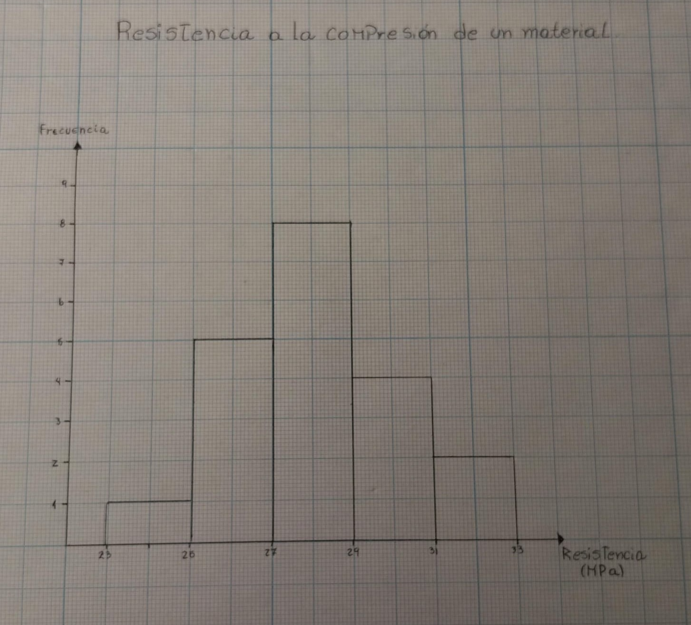
\includegraphics[width=0.7\textwidth]{grafico_mano.png}
\caption{Histograma de distribución de resistencia a la compresión realizado a mano.}
\label{fig:grafico-mano}
\end{figure}

En la Fig. \ref{fig:grafico-python} puede verse la representación gráfica de los mismos datos, elaborada utilizando el paquete Matplotlib de Python.

\begin{figure}[h!]
\centering
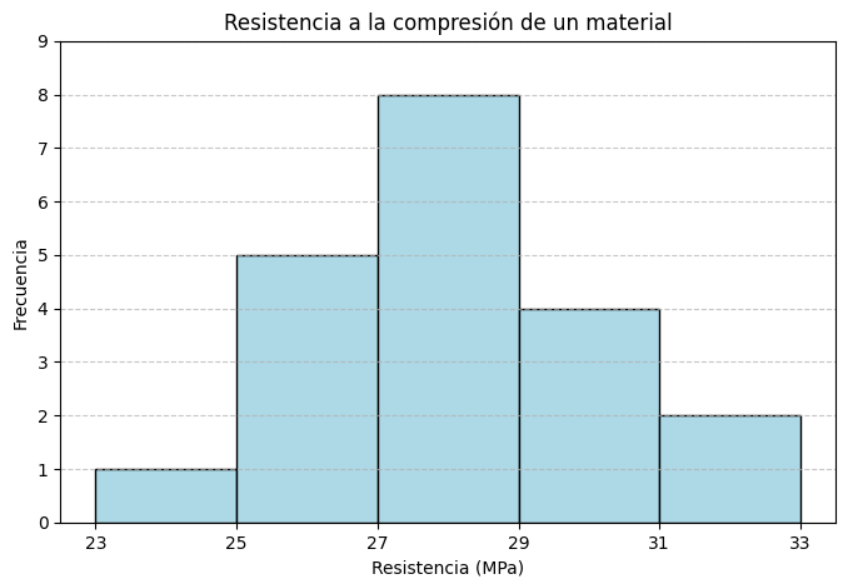
\includegraphics[width=0.7\textwidth]{grafico_python.png}
\caption{Histograma de distribución de resistencia a la compresión elaborado en Python.}
\label{fig:grafico-python}
\end{figure}

\subsubsection{Descripción y análisis}

Los gráficos presentan la distribución de frecuencias de la resistencia a la compresión agrupada en intervalos de ancho 2 MPa (con límites en 23, 25, 27, 29, 31 y 33 MPa). En el eje horizontal se ubica la resistencia a la compresión, mientras que en el eje vertical se representa la frecuencia absoluta de cada intervalo. Al analizar las figuras, se aprecia un comportamiento unimodal con una mayor concentración de datos en la zona central, disminuyendo progresivamente hacia los extremos. Específicamente, el intervalo modal es el comprendido entre 27 y 29 MPa, el cual alcanza una frecuencia máxima de 8 muestras. Este valor es el central representativo de la resistencia típica del material analizado. 

Al comparar ambas representaciones, se observa total coincidencia en la altura de las barras y la escala de los ejes; el uso de Python entrega una visualización más precisa, mientras que el gráfico manual confirma la correcta clasificación de los datos. Finalmente, debido a que se trata de la distribución de frecuencias de una sola variable continua (y no de una relación bivariada), no corresponde aplicar un ajuste lineal a este conjunto de datos.

\section{Análisis y conclusiones}

En esta sección, resuman brevemente lo realizado en cada una de las tres partes del informe. Indiquen qué se hizo y cuál fue el propósito de cada actividad, haciendo referencia a las secciones, tablas y ecuaciones correspondientes cuando sea necesario. No es necesario volver a enunciar todos los datos o repetir los procedimientos detallados anteriormente. El resumen puede realizarse en un solo párrafo o en tres párrafos distintos, uno para cada parte.

Luego del resumen de las actividades, respondan las preguntas de análisis planteadas en las tres partes de la guía. Pueden presentar todas las respuestas en un solo texto o separarlas en tres párrafos, uno para cada actividad. En cada respuesta, no se limiten a indicar un resultado: expliquen el razonamiento que utilizaron para llegar a él y relacionen sus conclusiones con los datos, cálculos y gráficos obtenidos durante el trabajo. Las respuestas a las preguntas de análisis deben estar integradas en el texto, conectando ideas mediante conectores lógicos. Eviten presentar las respuestas de manera aislada, como en formato pregunta-respuesta.

Finalmente, incluyan las principales conclusiones a las que llegaron como grupo. Estas deben sintetizar los aprendizajes obtenidos a partir de las actividades realizadas y destacar los aspectos que consideren más relevantes respecto de la medición de magnitudes físicas, el tratamiento de datos y su representación gráfica. Cuando corresponda, indiquen también las principales limitaciones o fuentes de incertidumbre que hayan identificado durante el trabajo.

Las conclusiones deben basarse en los resultados obtenidos por el grupo. \textbf{No incluyan citas bibliográficas en esta sección}.

\textbf{\underline{Extensión máxima del informe:} indefinida}.

\begin{thebibliography}{99}

\bibitem{libro} Nombre del autor. \textit{Título del libro}. Año.

\bibitem{apunte} Nombre del profesor. \textit{Nombre del curso}. Semestre y año en el que fue entregado el apunte.

\bibitem{web} TikTok de @usuario. Disponible en: \url{https://www.tiktok.com/}. 

\end{thebibliography}

\end{document}
